\documentclass{article}

\usepackage{graphicx}
\usepackage{subfigure}
\usepackage[hypcap]{caption}
\usepackage{listings}
\usepackage{float}
\floatstyle{plaintop}
\restylefloat{table}

\title{Experimental Design and Data Analysis: Assignment 2}
\author{Andrew Bedard(2566978) \& Simone van Gompel(2567525) \\ Group 19}

\begin{document}

  \maketitle

  \section{Exercise 1}
  \subsection*{1}
  Using data from \textit{peruvians.txt} we use the pairs command in R to produce a scatter plot of every variable against every other. The result can be seen in Fig:\ref{fig:Pairs}. From this figure, the variables age and weight seem to have a linear relationship, which would suggest that they are correlated.

    \begin{figure}[!htb]
      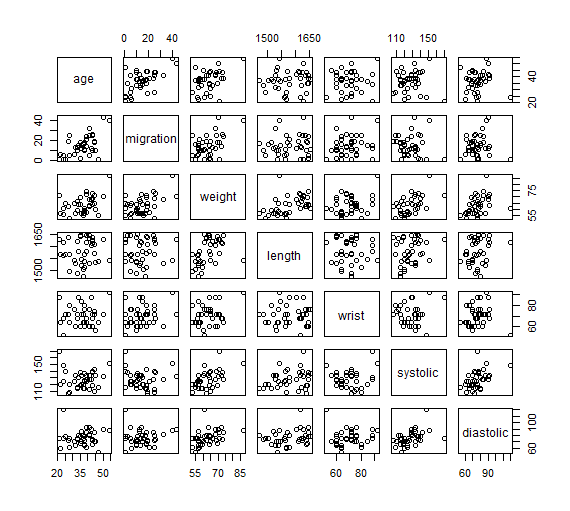
\includegraphics[scale=0.6]{../results/Pairs.png}
      \caption{Pairwise scatterplots of the dataset peruvians}
      \label{fig:Pairs}
    \end{figure}
    
    \subsection*{2}
    Using the Pearson (rank?) correlation test for all variables against migration we obtain the following results:
    \newline
    \begin{tabular}{|c|c|c|c|c|c|c|c|}
    \hline 
     & age & migration & weight & length & wrist & systolic & diastolic \\ 
    \hline 
    migration & 0.47605753 & 1 & 0.35069559 & 0.08458432 & 0.21934983 & -0.16842856 & 0.07514098 \\ 
    \hline 
    \end{tabular} 
    
    Age was the most obviously correlated variable between migration when the pairs scatter plots (Fig: \ref{fig:Pairs}), and age is the most correlated variable with migration.
    Weight is the second most correlated variable with migration, ...
    
    \section{Exercise 2}
    \subsection*{1}
    
    Two sample t-test assumes that both samples come from a normal population. 
    t-test: p-value =0.05375. The 95\% confidence interval is [-4.7405,559.5859] with mean of x = 441.9846 mean of y = 164.5619.
    We accept the null hypothesis
    The Mann-Whitney test: W=473, p-value = 0.01383
    we reject the null hypothesis
    Kolmogorov-Smirnov test: D = 0.4231, p-value = 0.01905
    we reject the null hypothesis
    
    \begin{figure}[!htb]
      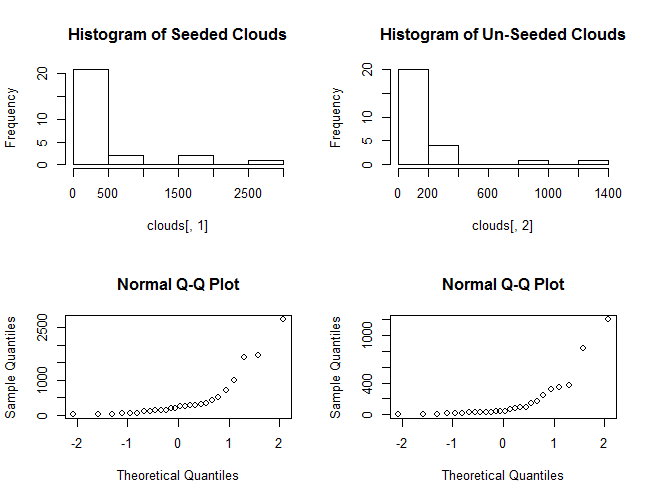
\includegraphics[scale=0.4]{../results/2_1.png}
      \caption{clouds}
      \label{fig:clouds}
    \end{figure}
    
    Two sample t-test
    
    \subsection*{2}
    t-test: t=2.4246, p-value = 0.01956, 95\% confidence interval [1.2021,13.0713], mean x=17.068, mean y= 9.9313
    Mann-Whitney test: The Mann-Whitney test: W=473, p-value = 0.01383
    Kolmogorov-Smirnov test: D = 0.4231, p-value = 0.01905
    
    \begin{figure}[!htb]
      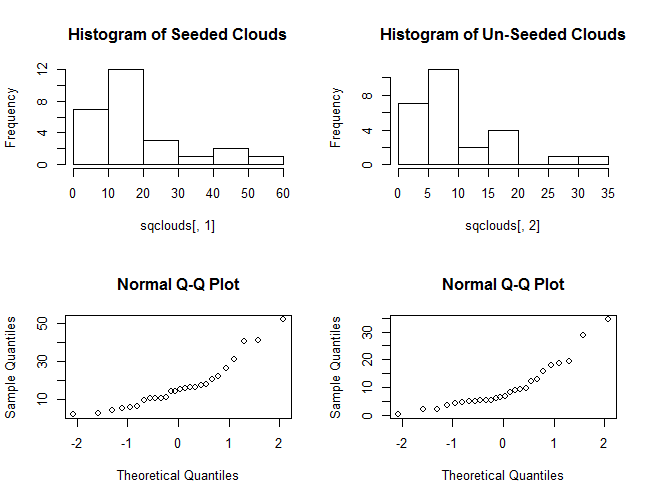
\includegraphics[scale=0.4]{../results/2_2.png}
      \caption{sq(clouds)}
      \label{fig:sq(clouds)}
    \end{figure}
    
    \subsection*{3}
    t-test: t=2.5968, p-value=0.0124, 95\% [0.2196,1.7236], mean x = 3.8789, mean y = 2.9073
    Mann-Whitney test: The Mann-Whitney test: W=473, p-value = 0.01383
    Kolmogorov-Smirnov test: D = 0.4231, p-value = 0.01905
    
    \begin{figure}[!htb]
      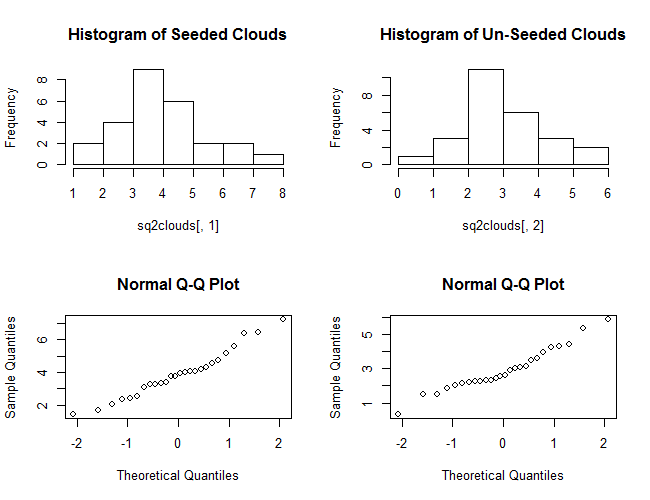
\includegraphics[scale=0.4]{../results/2_3.png}
      \caption{sq(sq(clouds))}
      \label{fig:sqsqclouds}
    \end{figure}
    
    \begin{figure}[!htb]
      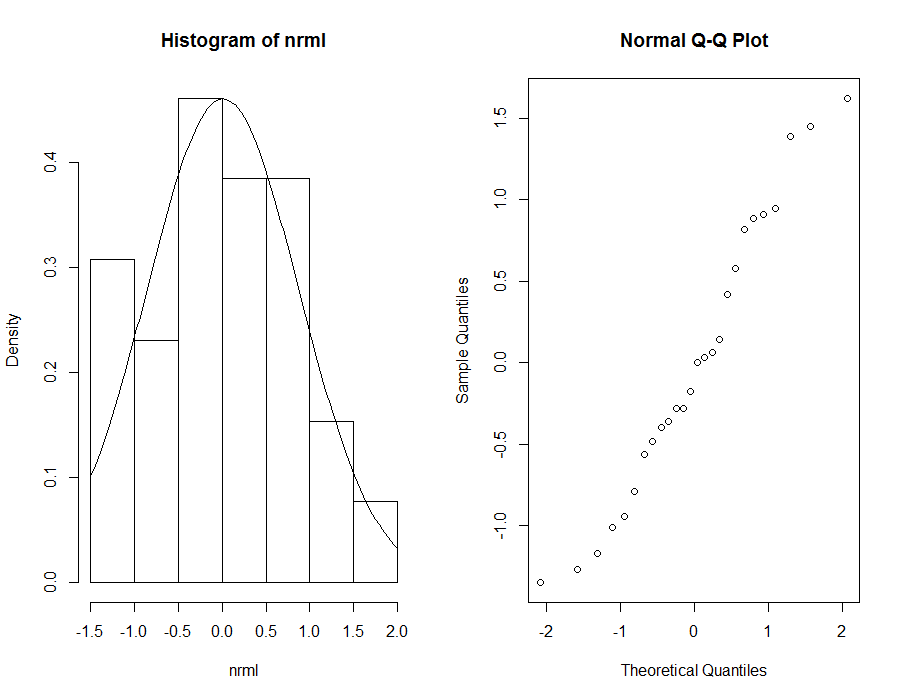
\includegraphics[scale=0.3]{../results/2_3_nrml.png}
      \caption{normal}
      \label{fig:normal}
    \end{figure}
    
    \section{3}
    \subsection*{1}
    \begin{figure}[!htb]
    \centering
      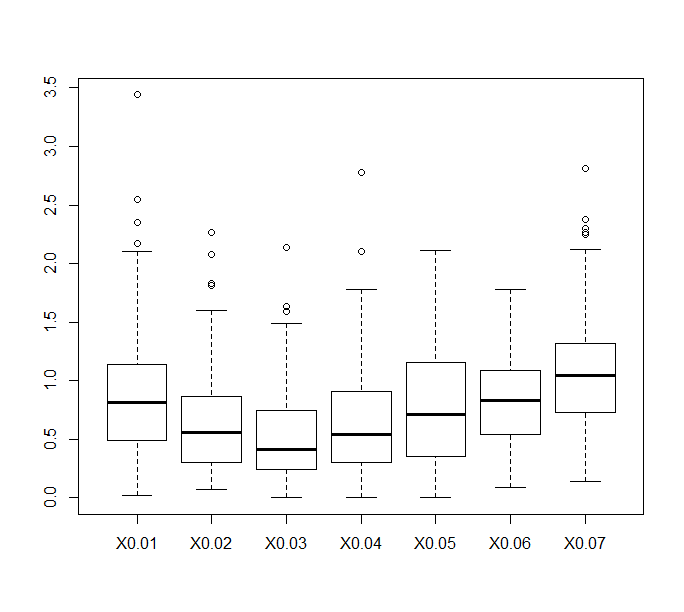
\includegraphics[scale=0.3]{../results/3_1.png}
      \caption{box}
      \label{fig:box}
    \end{figure}
    \subsection*{2}
    \begin{figure}[!htb]
      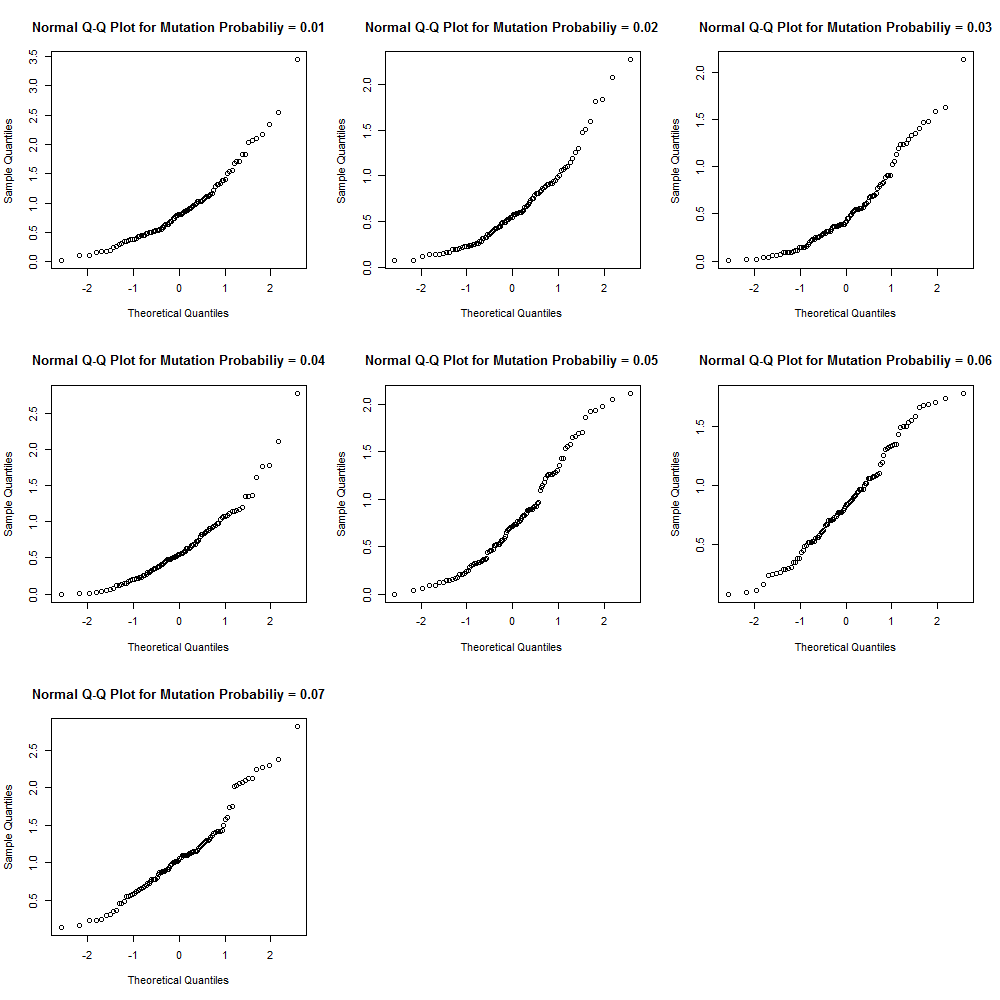
\includegraphics[scale=0.4]{../results/3_2_1.png}
      \caption{qq-genal}
      \label{fig:qq-genal}
    \end{figure}
    \begin{figure}[!htb]
    \centering
      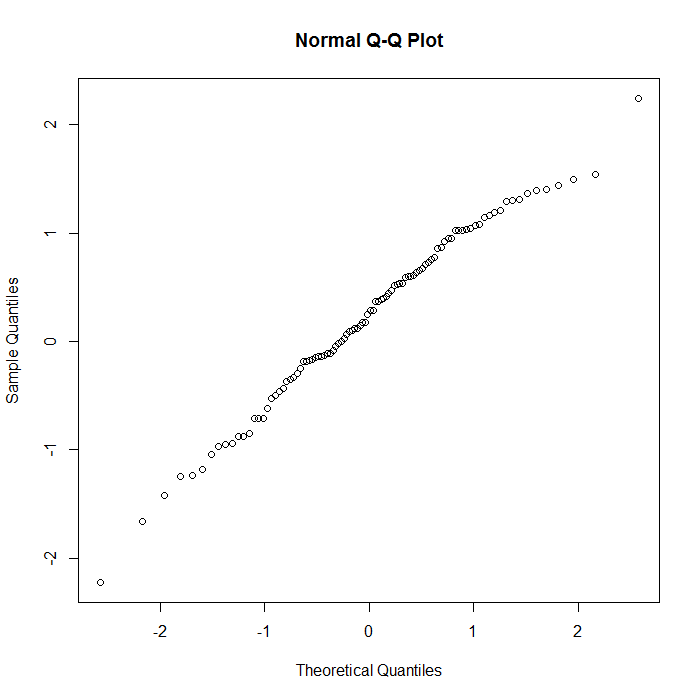
\includegraphics[scale=0.3]{../results/3_2_2.png}
      \caption{qq-nrml}
      \label{fig:qq-nrml}
    \end{figure}
    
    No
    \subsection*{3}
    \begin{figure}[!htb]
      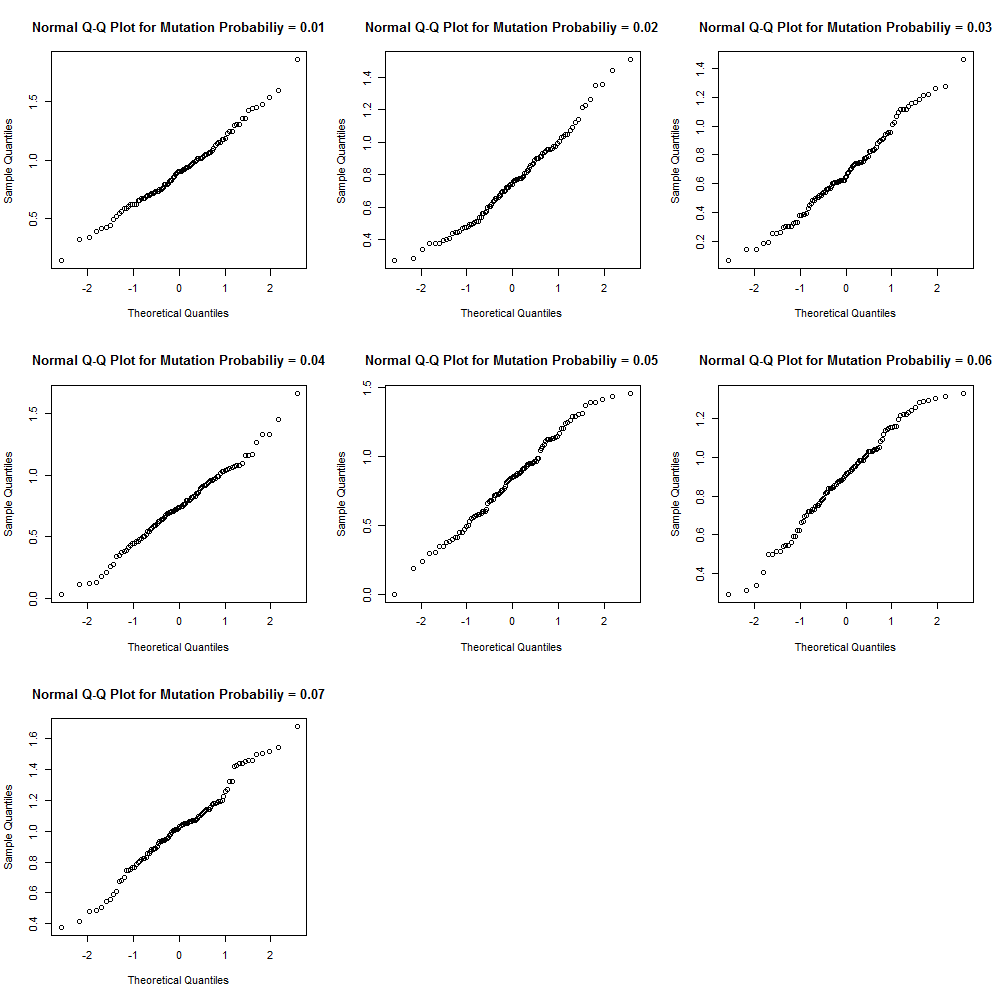
\includegraphics[scale=0.4]{../results/3_3.png}
      \caption{qq-sq(genal)}
      \label{fig:qq-sqgenal}
    \end{figure}
    
    Yes
    \subsection*{4}
    
    Using sq(genal) we find a p-value of 2.2e-16, therefore we reject the null hypothesis
    \subsection*{5}
    Based on summary(sqaov) X=0.03 is the best, because 0.9033-0.2227 is the smallest value, and we are estimating the smallest value obtained from an optimization where smaller is better.
    \subsection*{6}
    \begin{figure}[!htb]
    \centering
      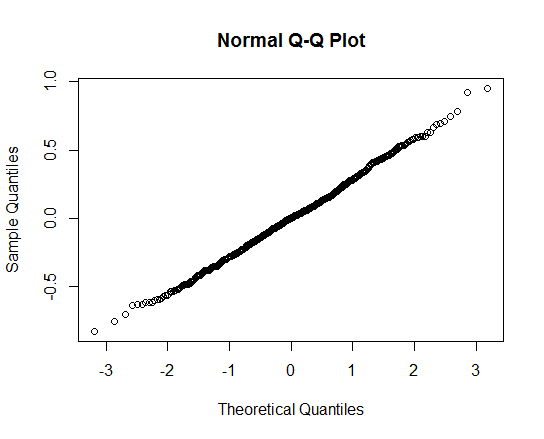
\includegraphics[scale=0.4]{../results/3_6.png}
      \caption{qq-resid}
      \label{fig:qq-resid}
    \end{figure}
    
    \section{4}
    \subsection*{1}
    \begin{figure}[!htb]
    \centering
      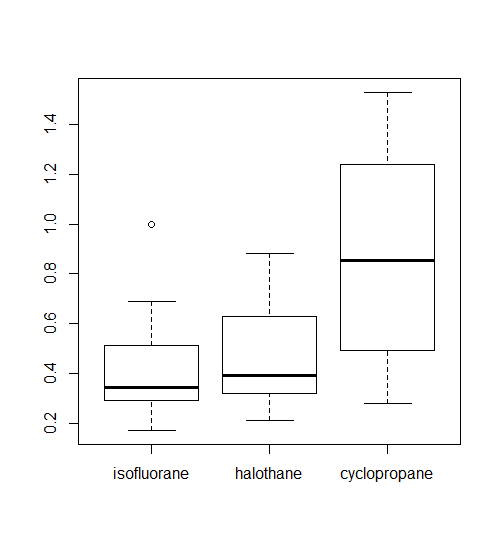
\includegraphics[scale=0.4]{../results/4_1.png}
      \caption{dog box}
      \label{fig:dbox}
    \end{figure}
    \subsection*{2}
    \begin{figure}[!htb]
    \centering
      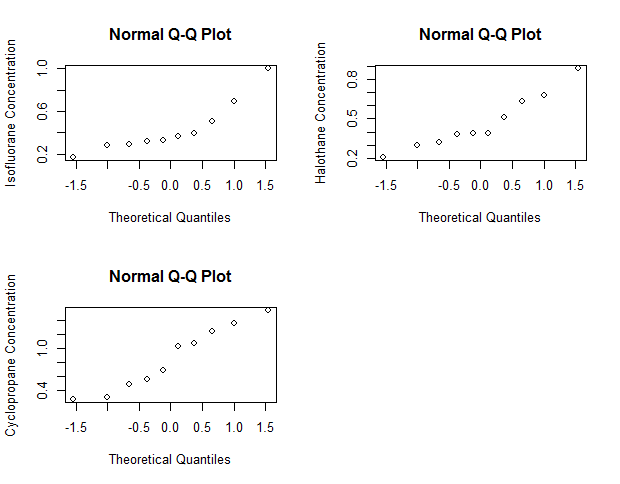
\includegraphics[scale=0.6]{../results/4_2.png}
      \caption{qq dog}
      \label{fig:qq dog}
    \end{figure}
    
    No, the sample sizes are far too small to reasonably judge whether or not they are normal populations.
    \subsection*{3}
    Reject the null, p-value 0.011, estimated value of Isofluorane: 0.4340, of Halothane: 0.469 and of Cyclopropane: 0.853
    \subsection*{4}
    The Kruskal-Wallis test for the same hypothesis gives a p-value of 0.05948, thus we do not reject the null hypothesis. 
    \subsection*{5}
    The differences between the 1-way Anova and the Kruskal-Wallis test could be explained by our initial assumption that the 3 samples represented in the data do not in fact come from a normal population, because 1-way Anova assumes that we are sampling from normal populations this could produce conflicting results, though as we see in Figure \ref{fig:dog-resid} the residuals do not deviate from the normal significantly.
    It is perhaps more compelling that the differences between the 1-way Anova and the Kruskal-Wallis are due to the fact that 1-way Anova assumes our populations have equal population variances, and as is observed in Figure \ref{fig:dbox}, they are obviously not equal.
    \begin{figure}[!htb]
    \centering
      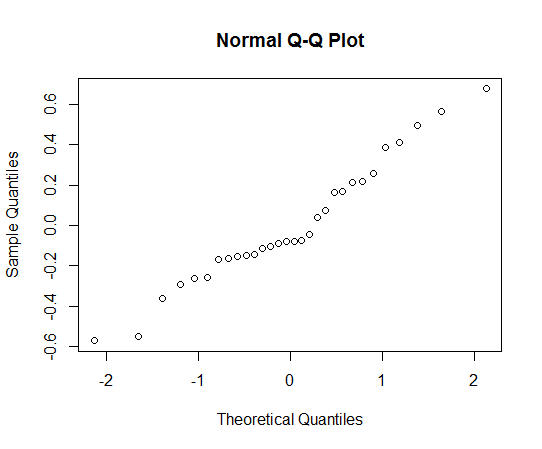
\includegraphics[scale=0.4]{../results/4_5.png}
      \caption{dog-resid}
      \label{fig:dog-resid}
    \end{figure}
    
    \section{R-Code}
    \subsection{Exercise 1}\label{sec:RE1}
      \begin{lstlisting}[language=R]
      #1.1
peru = read.table("peruvians.txt", header=T)
peru = peru[,-c(5,6,7)]
pairs(peru)

#1.2
#This shows the spearman rank correlation against all variables
correl_s = cor(peru, method="spearman")

correl_s[2, ]
      \end{lstlisting}
    \subsection{Exercise 2}\label{sec:RE2}
      \begin{lstlisting}[language=R]
      #2.1
clouds = read.table("clouds.txt", header=T)
len = length(clouds[,1])
nrml = rnorm(len)

#Histograms,boxplots,qqplots to see if data is normal
par(mfrow=c(2,2))
hist(clouds[,1])
hist(clouds[,2])
qqnorm(clouds[,1])
qqnorm(clouds[,2])
#These graphs should show the data is not normal

#Two sample t-test 
t.test(clouds[ ,1],clouds[ ,2])
#Mann-Whitney test
wilcox.test(clouds[ ,1],clouds[ ,2])
#Kolmogorov-Smirnov test
ks.test(clouds[,1],clouds[,2])

#2.2
sqclouds = sqrt(clouds)

#Histograms,boxplots,qqplots to see if data is normal
par(mfrow=c(2,2))
hist(sqclouds[,1])
hist(sqclouds[,2])
qqnorm(sqclouds[,1])
qqnorm(sqclouds[,2])
#These graphs should show the data is not normal

#Two sample t-test 
t.test(sqclouds[ ,1],sqclouds[ ,2])
#Mann-Whitney test
wilcox.test(sqclouds[ ,1],sqclouds[ ,2])
#Kolmogorov-Smirnov test
ks.test(sqclouds[,1],sqclouds[,2])

#2.3
sq2clouds = sqrt(sqclouds)

#Histograms,boxplots,qqplots to see if data is normal
par(mfrow=c(2,2))
hist(sq2clouds[,1])
hist(sq2clouds[,2])
qqnorm(sq2clouds[,1])
qqnorm(sq2clouds[,2])
#These graphs should show the data is not normal

#Two sample t-test
t.test(sq2clouds[ ,1],sq2clouds[ ,2])
#Mann-Whitney test
wilcox.test(sq2clouds[ ,1],sq2clouds[ ,2])
#Kolmogorov-Smirnov test
ks.test(sq2clouds[,1],sq2clouds[,2])

par(mfrow=c(1,2))
hist(nrml, prob=TRUE)
curve(dnorm(x,mean=mean(nrml),sd=sd(nrml)), add=TRUE)
qqnorm(nrml)
      \end{lstlisting}
    \subsection{Exercise 3}\label{sec:RE3}
      \begin{lstlisting}[language=R]
#3.1
genal = read.table("genal.txt", header=T)
len=length(genal[,1])
nrml=rnorm(len)

par(mfrow=c(1,1));boxplot(genal)

#3.2
#Loops through, creating QQ-plot for each mutation probability
par(mfrow=c(3,3))
for (i in 1:7) {
  qqnorm(genal[,i],
         main =paste("Normal Q-Q Plot for Mutation Probabiliy =",
                     i/100))
}
#qqplot of normal random sample of same size as genal[,i]
par(mfrow=c(1,1));qqnorm(nrml)
#3.3
sqgenal=sqrt(genal)

#Loops through, creating QQ-plot for each mutation probability
par(mfrow=c(3,3))
for (i in 1:7) {
  qqnorm(sqgenal[,i],
         main =paste("Normal Q-Q Plot for Mutation Probabiliy =",
                     i/10))
}

#3.4

#Create data-frames for the origional genal data, 
#and the squareroot genal data
sqframe=data.frame(yield=as.vector(as.matrix(sqgenal)),
                      variety=factor(rep(1:7,each=100)))

sqaov=lm(yield~variety,data=sqframe)
anova(sqaov)

#3.5
summary(sqaov)

#3.6
par(mfrow=c(1,1));qqnorm(residuals(sqaov))

      \end{lstlisting}
    \subsection{Exercise 4}\label{sec:RE4}
      \begin{lstlisting}[language=R]
      #4.1

dogs = read.table("dogs.txt", header=T)
len=length(dogs[,1])
boxplot(dogs)

#4.2
par(mfrow=c(2,2))
qqnorm(dogs[,1],ylab="Isofluorane Concentration")
qqnorm(dogs[,2],ylab="Halothane Concentration")
qqnorm(dogs[,3],ylab="Cyclopropane Concentration")

#4.3
dogframe = data.frame(yield=as.vector(as.matrix(dogs)),
                      variety=factor(rep(1:3,each=10)))
dogaov=lm(yield~variety,data=dogframe)
anova(dogaov)
summary(dogaov)

#Calculate expected value
u1=0.4340; 
u2=0.0350+u1
u3=0.4190+u1

print(u1,u2,u3)
#4.4

attach(dogframe)
kruskal.test(yield,variety)
par(mfrow=c(1,1));qqnorm(dogaov$residuals)

#Calculate and print population variances
for (i in 1:3){
  print(sum((dogs[,i]-mean(dogs[,i]))^2)/(len-1))
}
      \end{lstlisting}
\end{document}